\section{Unified Process}
Unified Process forkortes også UP og er en systemudviklingsmetode, der blev udviklet i slutningen af 90'erne af Ivar Jacobsen, Grady Booch og James Rumbaugh. I Unified Process gøres der brug af iterationer som projektet skal udvikles i, et større projekts iterationer varer typsik 2 til 6 uger. Når man udvikler et stykke software med Unified Process skal man igennem fire faser. Inception fasen hvor man forbereder hvilke ting der skal laves og danner et overblik over de forskellige opgaver der skal løses. Den næste fase kaldes Elaboration, i denne fase udvikles de centrale dele af programmet samt de dele der er vurderet sværest at lave, da de skal udvikles tidligt i processen så de ikke bliver udviklet under tidspres. Elaboration fasen er længere end Inception fasen, når fasen er slut vil kerneelementerne af programmet være udviklet. Efter Elaboration kommer Construction fasen, her udvikles de elementer i systemet som skal til for at programmet bliver færdigt, samt at programmet testes løbende igennem fasen. Construction fasen består af mindre iterationer, og det er også fasen hvor man begynder at alpha teste programmet. Udover tests bliver der også udført performance tuning og dokumentation i Construction fasen. Sidst men ikke mindst er der Transition fasen, dette er fasen hvor programmet bliver udgivet, Transition fasen kan have flere iterationer hvor programmet får anmeldelser og feedback inden det bliver udgivet. \newline
\newline
\subsection{Vores Forløb med Unified Process}
I processen med at skabe Unreal Breakout har det ikke været muligt at nå alt som Unified Process indebærer, dog har det stadig været muligt at følge det. Inception fasen blev fuldført med objekt orienteret analyse og design, samt udarbejdelsen af et Gantt-chart, som estimere tiden der skal bruges på de forskellige dele af projektet. Der blev også udarbejdet en risikovurdering i inceptionfasen som skulle vurdere de forskellige risici der er ved at lave et større projekt, samt sætte tal på hvor alvorlige problemerne der kan opstå er. \newline
I Elaboration fasen blev det lavet én iteration for at få grundelementerne i spillet lavet, iterationen varede i alt 5 dage og resulterede i at spillet blev til et spilbart. Der blev i fasen taget højde for hvilke elementer der ville være tidskrævende at udvikle og disse elementer blev lavet først i fasen. \newline
Efter Elaboration fasen begyndte Construction fasen. Construction fasen bestod af én kort iteration hvor der blev fortaget en Blackbox test på programmet samt rettet småfejl. 
\newline
Transition fasen blev ikke taget i brug i processen med at lave Unreal Breakout da produktet ikke skulle leveres til en kunde og først får ekstern feedback til eksamen. 
 
\subsection{Fasediagram}

\begin{figure}
	\begin{center}
		\caption{UP Phasediagram.}
		\label{dia:upphase}
		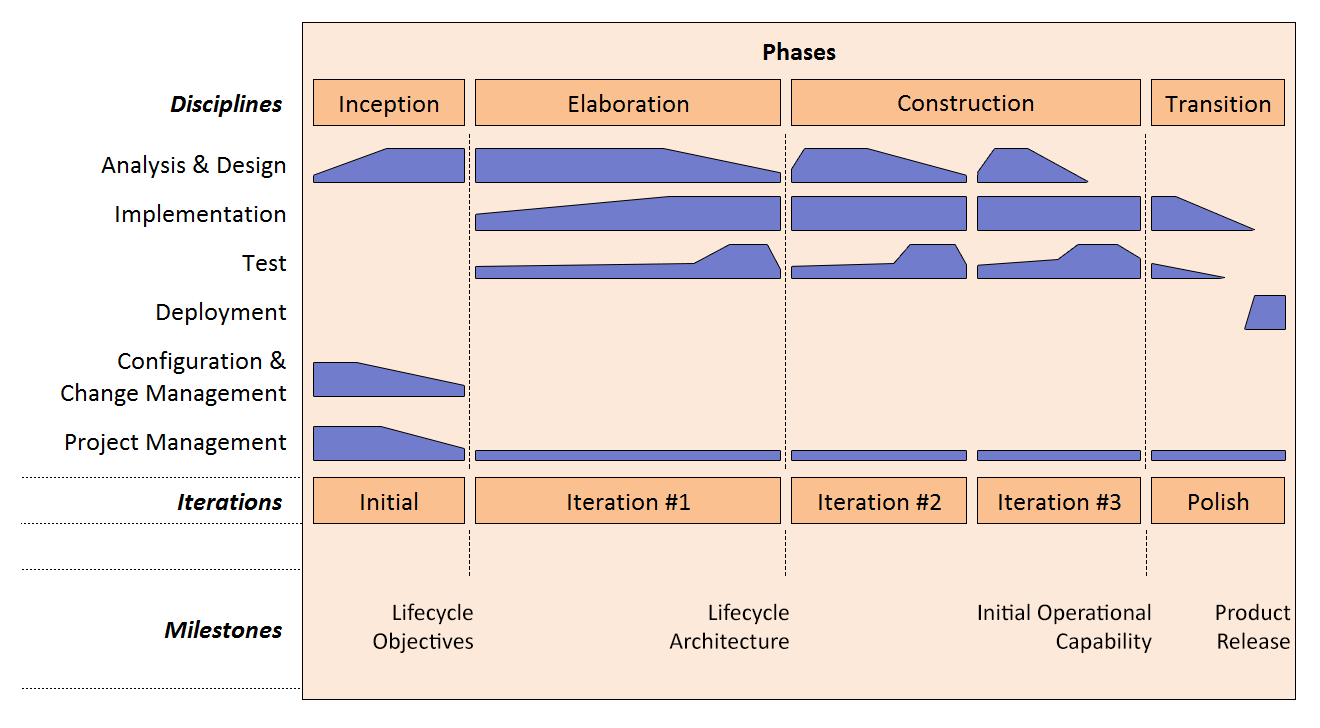
\includegraphics[width=0.98\linewidth]{pictures/up/up-phase}
	\end{center}
\end{figure}

\subsection{Risikoanalyse}
Som det kan ses i tabel \ref{tbl:risikoanalyse} er der udarbejdet en risikovurdering som kan hjælpe med at identificere steder som kan volde problemer for projektet. Disse risici kan være med til at gøre hele projektet længere hvis ikke man tager højde for dem på forhånd og indarbejder dem i sin tidsestimering.

\begin{table}[]
	\centering
	\caption{Risikovurdering}
	\label{tbl:risikoanalyse}
	\begin{tabular}{|l|l|l|l|}
		\hline
		\multicolumn{1}{|c|}{\textbf{Risiko}} & \multicolumn{1}{c|}{\textbf{Risikoværdi}} & \multicolumn{1}{c|}{\textbf{Alvor af problem}} & \multicolumn{1}{c|}{\textbf{Risikotal}} \\ \hline
		Sygdom & 80\% & 2/10 & 80 * 2 = 160 \\ \hline
		Ændringer & 10\% & 6/10 & 10 * 6 = 60 \\ \hline
		Tekniske problemer & 90\% & 7/10 & 90 * 7 = 630 \\ \hline
		Fejlestimering & 30\% & 9/10 & 30 * 9 = 270 \\ \hline
		Internet nedbrud & 10\% & 9/10 & 10 * 9 = 90 \\ \hline
	\end{tabular}
\end{table}

Der er taget højde for at et gruppemedlem har ondt i ryggen og der ikke altid kan arbejdes i det normale tidsrum. Da gruppen arbejder med flextid og mange af opgaverne ikke kræver konstant samarbejde er det vurderet at risikoen er høj, men alvoren når det sker ikke har den store påvirkning. Der er også en risiko for almindelig sygdom, men igen er alvoren lav på grund af flextid og hjemmearbejde.

Det kan også hænde at der skal laves en ændring i gamedesignet, men da det er et meget simpelt spil er der nok ikke stor risiko for at det vil ske. Hvis en ændring sker skal der udvikles ny funktionalitet. Da spillet er forholdsvis simpelt vil det kræve noget, men nok ikke særligt komplekst arbejde.

Tekniske problemer vil højest sandsynligt opstå da udviklerne i gruppen alle er nye til Unreal Engine. Derfor vil der være meget søgning efter problemløsninger på internettet og Unreal Engines online dokumentation.

Selvom det ikke er sandsynligt at det vil ske, vil det være alvorligt med en fejlestimering. Grundet projektets omfang vil risikoværdien være lav, da planlægning er nem at overskue. Er der fejlestimering er det selvsigende at dette får kraftig indflydelse på tidsplanen.
 
\subsection{Ganttdiagram}

